\section*{Exercice 167 --  PFS}
% CCS TSI 2015

\setcounter{exo}{0}

Le mécanisme représenté schématiquement ci-dessus est destiné à assurer le levage d’une charge liée au coulisseau \textbf{(3)} au moyen d’un levier à excentrique \textbf{(1)} et d’un balancier \textbf{(2)}.

\begin{center}
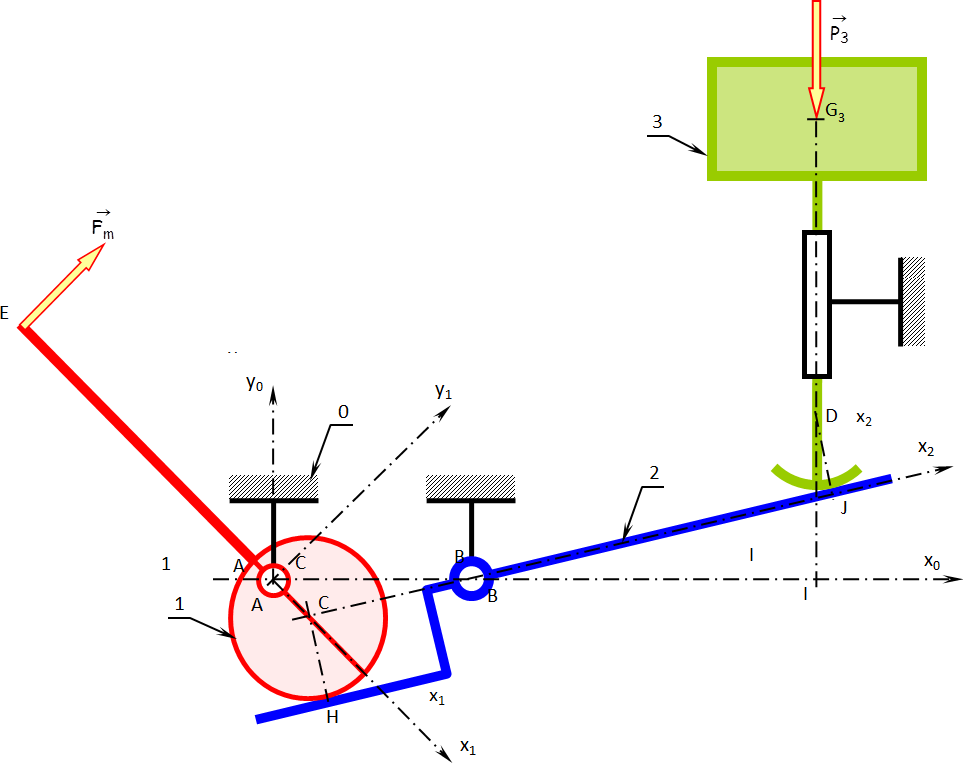
\includegraphics[width=\linewidth]{048_01}
%\textit{}
\end{center}
\begin{obj}
Objectif : Dans cette étude, on va mettre en évidence l’influence du frottement sur l’équilibre d’un système.
\end{obj}

On note  $\vect{P_3}$ le poids de la charge appliquée sur le coulisseau et $\vect{F_m}$ l’effort appliqué en $E$ par l’opérateur sur le levier à excentrique \textbf{(1)}.

\subsection*{Paramétrage géométrique}
$\vect{AB}=L_0\vect{x_0}$; 
$\vect{AE}=-L_1\vect{x_1}$; 
$\vect{BI}=d_0\vect{x_0}$; 
$\vect{AC}=e_1\vect{x_1}$; 
$\vect{HC}=R_1\vect{y_2}$; 
$\vect{BJ}=\lambda_{32}\vect{x_2}$; 
$\vect{ID}=\lambda_{30}\vect{y_0}$; 
$\vect{JD}=R_3\vect{y_2}$; 
$\left(\vect{x_0},\vect{x_1} \right)=\theta_{\left(1/0\right)}$; 
$\left(\vect{x_0},\vect{x_2} \right)=\theta_{\left(2/0\right)}$.
 	 	 	 	 

\subsection*{On suppose dans un premier temps que toutes les liaisons sont sans frottement.}

\subparagraph{}\textit{Réaliser le graphe de structure.}

\subparagraph{}\textit{En écrivant les équations associées à l’équilibre de chacune des pièces, établir la relation liant $F_m$ et $P_3$ à l’équilibre.   \textbf{On cherchera à écrire le minimum d'équations.}}
%\subparagraph{}\textit{Indiquer quelles sont les équations qui auraient pu permettre de trouver cette relation sans écrire tout le système d’équation.}
\subparagraph{}\textit{Pour quelle(s) valeur(s) particulières de $\theta_{1/0}$ l’équilibre est-il possible avec un effort $F_m$ nul ?}
